%%
% Copyright (c) 2017 - 2021, Pascal Wagler;
% Copyright (c) 2014 - 2021, John MacFarlane
%
% All rights reserved.
%
% Redistribution and use in source and binary forms, with or without
% modification, are permitted provided that the following conditions
% are met:
%
% - Redistributions of source code must retain the above copyright
% notice, this list of conditions and the following disclaimer.
%
% - Redistributions in binary form must reproduce the above copyright
% notice, this list of conditions and the following disclaimer in the
% documentation and/or other materials provided with the distribution.
%
% - Neither the name of John MacFarlane nor the names of other
% contributors may be used to endorse or promote products derived
% from this software without specific prior written permission.
%
% THIS SOFTWARE IS PROVIDED BY THE COPYRIGHT HOLDERS AND CONTRIBUTORS
% "AS IS" AND ANY EXPRESS OR IMPLIED WARRANTIES, INCLUDING, BUT NOT
% LIMITED TO, THE IMPLIED WARRANTIES OF MERCHANTABILITY AND FITNESS
% FOR A PARTICULAR PURPOSE ARE DISCLAIMED. IN NO EVENT SHALL THE
% COPYRIGHT OWNER OR CONTRIBUTORS BE LIABLE FOR ANY DIRECT, INDIRECT,
% INCIDENTAL, SPECIAL, EXEMPLARY, OR CONSEQUENTIAL DAMAGES (INCLUDING,
% BUT NOT LIMITED TO, PROCUREMENT OF SUBSTITUTE GOODS OR SERVICES;
% LOSS OF USE, DATA, OR PROFITS; OR BUSINESS INTERRUPTION) HOWEVER
% CAUSED AND ON ANY THEORY OF LIABILITY, WHETHER IN CONTRACT, STRICT
% LIABILITY, OR TORT (INCLUDING NEGLIGENCE OR OTHERWISE) ARISING IN
% ANY WAY OUT OF THE USE OF THIS SOFTWARE, EVEN IF ADVISED OF THE
% POSSIBILITY OF SUCH DAMAGE.
%%

%%
% This is the Eisvogel pandoc LaTeX template.
%
% For usage information and examples visit the official GitHub page:
% https://github.com/Wandmalfarbe/pandoc-latex-template
%%

% Options for packages loaded elsewhere
\PassOptionsToPackage{unicode}{hyperref}
\PassOptionsToPackage{hyphens}{url}
\PassOptionsToPackage{dvipsnames,svgnames*,x11names*,table}{xcolor}
%
\documentclass[
  12pt,
  paper=a4,
  ,captions=tableheading
]{scrartcl}
\usepackage{xeCJK}
% \setCJKmainfont{Source Han Serif}
\setCJKmainfont[AutoFakeBold=1.8]{教育部標準楷書}
\usepackage{amsmath,amssymb}
\usepackage{lmodern}
\usepackage{setspace}
\setstretch{1.2}
\usepackage{ifxetex,ifluatex}
\ifnum 0\ifxetex 1\fi\ifluatex 1\fi=0 % if pdftex
  \usepackage[T1]{fontenc}
  \usepackage[utf8]{inputenc}
  \usepackage{textcomp} % provide euro and other symbols
\else % if luatex or xetex
  \usepackage{unicode-math}
  \defaultfontfeatures{Scale=MatchLowercase}
  \defaultfontfeatures[\rmfamily]{Ligatures=TeX,Scale=1}
\fi
% Use upquote if available, for straight quotes in verbatim environments
\IfFileExists{upquote.sty}{\usepackage{upquote}}{}
\IfFileExists{microtype.sty}{% use microtype if available
  \usepackage[]{microtype}
  \UseMicrotypeSet[protrusion]{basicmath} % disable protrusion for tt fonts
}{}
\makeatletter
\@ifundefined{KOMAClassName}{% if non-KOMA class
  \IfFileExists{parskip.sty}{%
    \usepackage{parskip}
  }{% else
    \setlength{\parindent}{0pt}
    \setlength{\parskip}{6pt plus 2pt minus 1pt}}
}{% if KOMA class
  \KOMAoptions{parskip=half}}
\makeatother
\usepackage{xcolor}
\definecolor{default-linkcolor}{HTML}{A50000}
\definecolor{default-filecolor}{HTML}{A50000}
\definecolor{default-citecolor}{HTML}{4077C0}
\definecolor{default-urlcolor}{HTML}{4077C0}
\IfFileExists{xurl.sty}{\usepackage{xurl}}{} % add URL line breaks if available
\IfFileExists{bookmark.sty}{\usepackage{bookmark}}{\usepackage{hyperref}}
\hypersetup{
  pdftitle={Recognition of Fanout-free Functions},
  pdfauthor={107021129 黃明瀧},
  colorlinks=true,
  linkcolor=default-linkcolor,
  filecolor=default-filecolor,
  citecolor=default-citecolor,
  urlcolor=default-urlcolor,
  breaklinks=true,
  pdfcreator={LaTeX via pandoc with the Eisvogel template}}
\urlstyle{same} % disable monospaced font for URLs
\usepackage[margin=2.5cm,includehead=true,includefoot=true,centering,]{geometry}
% add backlinks to footnote references, cf. https://tex.stackexchange.com/questions/302266/make-footnote-clickable-both-ways
\usepackage{footnotebackref}
\usepackage{graphicx}
\makeatletter
\def\maxwidth{\ifdim\Gin@nat@width>\linewidth\linewidth\else\Gin@nat@width\fi}
\def\maxheight{\ifdim\Gin@nat@height>\textheight\textheight\else\Gin@nat@height\fi}
\makeatother
% Scale images if necessary, so that they will not overflow the page
% margins by default, and it is still possible to overwrite the defaults
% using explicit options in \includegraphics[width, height, ...]{}
\setkeys{Gin}{width=\maxwidth,height=\maxheight,keepaspectratio}
% Set default figure placement to htbp
\makeatletter
\def\fps@figure{htbp}
\makeatother
\setlength{\emergencystretch}{3em} % prevent overfull lines
\providecommand{\tightlist}{%
  \setlength{\itemsep}{0pt}\setlength{\parskip}{0pt}}
\setcounter{secnumdepth}{-\maxdimen} % remove section numbering

% Make use of float-package and set default placement for figures to H.
% The option H means 'PUT IT HERE' (as  opposed to the standard h option which means 'You may put it here if you like').
\usepackage{float}
\floatplacement{figure}{H}

\usepackage{amsthm}
\newtheorem*{thm}{定理}
\newtheorem*{lem}{引理}
\AtBeginDocument{%
\addto\captionsenglish{\renewcommand{\figurename}{圖}}
}
\makeatletter
\@ifpackageloaded{subfig}{}{\usepackage{subfig}}
\@ifpackageloaded{caption}{}{\usepackage{caption}}
\captionsetup[subfloat]{margin=0.5em}
\AtBeginDocument{%
\renewcommand*\figurename{Figure}
\renewcommand*\tablename{Table}
}
\AtBeginDocument{%
\renewcommand*\listfigurename{List of Figures}
\renewcommand*\listtablename{List of Tables}
}
\newcounter{pandoccrossref@subfigures@footnote@counter}
\newenvironment{pandoccrossrefsubfigures}{%
\setcounter{pandoccrossref@subfigures@footnote@counter}{0}
\begin{figure}\centering%
\gdef\global@pandoccrossref@subfigures@footnotes{}%
\DeclareRobustCommand{\footnote}[1]{\footnotemark%
\stepcounter{pandoccrossref@subfigures@footnote@counter}%
\ifx\global@pandoccrossref@subfigures@footnotes\empty%
\gdef\global@pandoccrossref@subfigures@footnotes{{##1}}%
\else%
\g@addto@macro\global@pandoccrossref@subfigures@footnotes{, {##1}}%
\fi}}%
{\end{figure}%
\addtocounter{footnote}{-\value{pandoccrossref@subfigures@footnote@counter}}
\@for\f:=\global@pandoccrossref@subfigures@footnotes\do{\stepcounter{footnote}\footnotetext{\f}}%
\gdef\global@pandoccrossref@subfigures@footnotes{}}
\@ifpackageloaded{float}{}{\usepackage{float}}
\floatstyle{ruled}
\@ifundefined{c@chapter}{\newfloat{codelisting}{h}{lop}}{\newfloat{codelisting}{h}{lop}[chapter]}
\floatname{codelisting}{Listing}
\newcommand*\listoflistings{\listof{codelisting}{List of Listings}}
\makeatother
\ifluatex
  \usepackage{selnolig}  % disable illegal ligatures
\fi
\newlength{\cslhangindent}
\setlength{\cslhangindent}{1.5em}
\newlength{\csllabelwidth}
\setlength{\csllabelwidth}{3em}
\newenvironment{CSLReferences}[2] % #1 hanging-ident, #2 entry spacing
 {% don't indent paragraphs
  \setlength{\parindent}{0pt}
  % turn on hanging indent if param 1 is 1
  \ifodd #1 \everypar{\setlength{\hangindent}{\cslhangindent}}\ignorespaces\fi
  % set entry spacing
  \ifnum #2 > 0
  \setlength{\parskip}{#2\baselineskip}
  \fi
 }%
 {}
\usepackage{calc}
\newcommand{\CSLBlock}[1]{#1\hfill\break}
\newcommand{\CSLLeftMargin}[1]{\parbox[t]{\csllabelwidth}{#1}}
\newcommand{\CSLRightInline}[1]{\parbox[t]{\linewidth - \csllabelwidth}{#1}\break}
\newcommand{\CSLIndent}[1]{\hspace{\cslhangindent}#1}

\title{Recognition of Fanout-free Functions}
\usepackage{etoolbox}
\makeatletter
\providecommand{\subtitle}[1]{% add subtitle to \maketitle
  \apptocmd{\@title}{\par {\large #1 \par}}{}{}
}
\makeatother
\subtitle{Presentation Report for Introduction to CAD}
\author{107021129 黃明瀧}
\date{2022-06-11}



%%
%% added
%%

%
% language specification
%
% If no language is specified, use English as the default main document language.
%

\ifnum 0\ifxetex 1\fi\ifluatex 1\fi=0 % if pdftex
  \usepackage[shorthands=off,main=english]{babel}
\else
    % Workaround for bug in Polyglossia that breaks `\familydefault` when `\setmainlanguage` is used.
  % See https://github.com/Wandmalfarbe/pandoc-latex-template/issues/8
  % See https://github.com/reutenauer/polyglossia/issues/186
  % See https://github.com/reutenauer/polyglossia/issues/127
  \renewcommand*\familydefault{\sfdefault}
    % load polyglossia as late as possible as it *could* call bidi if RTL lang (e.g. Hebrew or Arabic)
  \usepackage{polyglossia}
  \setmainlanguage[]{english}
\fi



%
% for the background color of the title page
%

%
% break urls
%
\PassOptionsToPackage{hyphens}{url}

%
% When using babel or polyglossia with biblatex, loading csquotes is recommended
% to ensure that quoted texts are typeset according to the rules of your main language.
%
\usepackage{csquotes}

%
% captions
%
\definecolor{caption-color}{HTML}{777777}
\usepackage[font={stretch=1.2}, textfont={color=caption-color}, position=top, skip=4mm, labelfont=bf, singlelinecheck=false, justification=raggedright]{caption}
\setcapindent{0em}

%
% blockquote
%
\definecolor{blockquote-border}{RGB}{221,221,221}
\definecolor{blockquote-text}{RGB}{119,119,119}
\usepackage{mdframed}
\newmdenv[rightline=false,bottomline=false,topline=false,linewidth=3pt,linecolor=blockquote-border,skipabove=\parskip]{customblockquote}
\renewenvironment{quote}{\begin{customblockquote}\list{}{\rightmargin=0em\leftmargin=0em}%
\item\relax\color{blockquote-text}\ignorespaces}{\unskip\unskip\endlist\end{customblockquote}}

%
% Source Sans Pro as the de­fault font fam­ily
% Source Code Pro for monospace text
%
% 'default' option sets the default
% font family to Source Sans Pro, not \sfdefault.
%
\ifnum 0\ifxetex 1\fi\ifluatex 1\fi=0 % if pdftex
    \usepackage[default]{sourcesanspro}
  \usepackage{sourcecodepro}
  \else % if not pdftex
    \usepackage[default]{sourcesanspro}
  \usepackage{sourcecodepro}

  % XeLaTeX specific adjustments for straight quotes: https://tex.stackexchange.com/a/354887
  % This issue is already fixed (see https://github.com/silkeh/latex-sourcecodepro/pull/5) but the
  % fix is still unreleased.
  % TODO: Remove this workaround when the new version of sourcecodepro is released on CTAN.
  \ifxetex
    \makeatletter
    \defaultfontfeatures[\ttfamily]
      { Numbers   = \sourcecodepro@figurestyle,
        Scale     = \SourceCodePro@scale,
        Extension = .otf }
    \setmonofont
      [ UprightFont    = *-\sourcecodepro@regstyle,
        ItalicFont     = *-\sourcecodepro@regstyle It,
        BoldFont       = *-\sourcecodepro@boldstyle,
        BoldItalicFont = *-\sourcecodepro@boldstyle It ]
      {SourceCodePro}
    \makeatother
  \fi
  \fi

%
% heading color
%
\definecolor{heading-color}{RGB}{40,40,40}
\addtokomafont{section}{\color{heading-color}}
% When using the classes report, scrreprt, book,
% scrbook or memoir, uncomment the following line.
%\addtokomafont{chapter}{\color{heading-color}}

%
% variables for title, author and date
%
\usepackage{titling}
\title{Recognition of Fanout-free Functions}
\author{107021129 黃明瀧}
\date{2022-06-11}

%
% tables
%

%
% remove paragraph indention
%
\setlength{\parindent}{0pt}
\setlength{\parskip}{6pt plus 2pt minus 1pt}
\setlength{\emergencystretch}{3em}  % prevent overfull lines

%
%
% Listings
%
%


%
% header and footer
%
\usepackage{fancyhdr}

\fancypagestyle{eisvogel-header-footer}{
  \fancyhead{}
  \fancyfoot{}
  \lhead[2022-06-11]{Recognition of Fanout-free Functions}
  \chead[]{}
  \rhead[Recognition of Fanout-free Functions]{2022-06-11}
  \lfoot[\thepage]{107021129 黃明瀧}
  \cfoot[]{}
  \rfoot[107021129 黃明瀧]{\thepage}
  \renewcommand{\headrulewidth}{0.4pt}
  \renewcommand{\footrulewidth}{0.4pt}
}
\pagestyle{eisvogel-header-footer}

%%
%% end added
%%

\begin{document}

%%
%% begin titlepage
%%
\vspace*{-1\baselineskip}
{\LARGE \textbf{\thetitle}}\\[0.5\baselineskip]
{\color{gray}\Large Presentation Report for Introduction to
CAD\hfill{\large \theauthor}}
\vspace{-0.5\baselineskip}

%%
%% end titlepage
%%



\hypertarget{ux7c21ux4ecb}{%
\section{簡介}\label{ux7c21ux4ecb}}

這篇論文{[}1{]}討論了有效率地判別布林函數是否為Fanout-less(無扇出)的方法。作者基於原有的演算法,利用Disappearance(消失)性質與Adjacency(相鄰)性質之間的關係,設計出了更高效率的演算法,並以實驗證明該演算法的優勢。

\hypertarget{ux5e38ux7528ux7b26ux865fux8207ux554fux984cux5b9aux7fa9}{%
\section{常用符號與問題定義}\label{ux5e38ux7528ux7b26ux865fux8207ux554fux984cux5b9aux7fa9}}

\begin{description}
\item[Fanout-less]
布林函式\(f(X)\)為fanout-less的,若且唯若存在一\(f\)的表示方法,使得\(X=\{x_1, \dots, x_n\}\)中每個元素在\(f\)中出現恰一次。

值得一提的是,在{[}2{]}中, fanout-free有一個等價的遞迴定義:

\begin{enumerate}
\def\labelenumi{\arabic{enumi}.}
\tightlist
\item
  Constant與\(x\)及\(\overline{x}\)為fanout-free。
\item
  兩個fanout-free functions
  \(f_1(X_1)\)與\(f_2(X_2)\),其中\(X_1\cap X_2 = \emptyset\),經過AND/OR/NOT運算後仍為fanout-free。
\end{enumerate}
\item[Cofactor]
布林函式\(f(X)\)對於\(x_i=c\)(此處\(c=0\)或\(c=1\))的cofactor,代表將\(f\)中\(x_i\)代入值\(c\)所得之新的布林函式。本文中記作\(f(x_i=c)\)。
\item[Adjacency]
布林函式\(f(X)\)中兩個變數\(x_i,x_j\in X\)為adjacent,若且唯若\(f(x_i=c) = f(x_j=c)\)。本文中記作\(x_i =_a x_j\)。

此關係在其他文獻中被證明為集合\(X\)上的一等價關係,因此\(=_a\)將集合\(X\)劃分為一或多個類,稱為adjacency
classes。
\item[Disappearance]
變數\(x\)消失於(disappears
in)布林函式\(f(X)\),若且唯若\(f\)之值不受\(x\)影響。
\end{description}

\hypertarget{jphux6f14ux7b97ux6cd5}{%
\section{JPH演算法}\label{jphux6f14ux7b97ux6cd5}}

JPH演算法為John P.
Hayes在{[}2{]}中提出的fanout-free判別演算法。該算法主要利用了adjacency關係與以下定理(該論文中定理4)。

\begin{thm}

以adjacency關係將$f(X)$的輸入變數集合$X$劃分為等價類$X_1, X_2, \dots, X_m$,
則存在$\phi_1(X_1), \phi_2(X_2), \dots, \phi_m(X_m)$以及函式$F$,其中$\phi_i$為AND或OR函式,
使得$f(X) = F(\phi_1(X_1), \phi_2(X_2), \dots, \phi_m(X_m))$。

\end{thm}

JPH演算法執行過程為一個迴圈,每次迭代都利用上述定理,如圖~\ref{fig:decomp}所示,將當前的輸入函式\(f_i\)之輸入\(X_i\)劃分為adjacency
classes後,從\(f\)分離出\(\phi_{i_1}, \dots, \phi_{i_r}\)等邏輯閘,再以檢視真值表的方式來建構出剩餘部分的新函式\(f_{i+1}\)。

\begin{figure}
\hypertarget{fig:decomp}{%
\centering
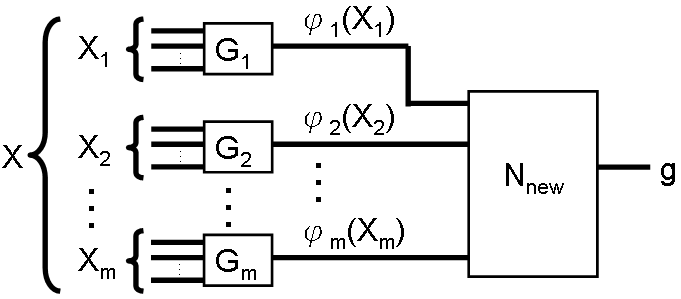
\includegraphics[width=0.55\textwidth,height=\textheight]{./resources/adj-decomp.png}
\caption{利用adjacency關係進行函式的拆解}\label{fig:decomp}
}
\end{figure}

圖~\ref{fig:jph}展示了JPH演算法的流程。注意此演算法在每次迭代中,都需要實行兩兩cofactor之間的等效性檢查,以確認\(f_i\)的輸入變數之間的adjacency關係。本篇論文提出了不需等效性檢查的替代做法。

\begin{figure}
\hypertarget{fig:jph}{%
\centering
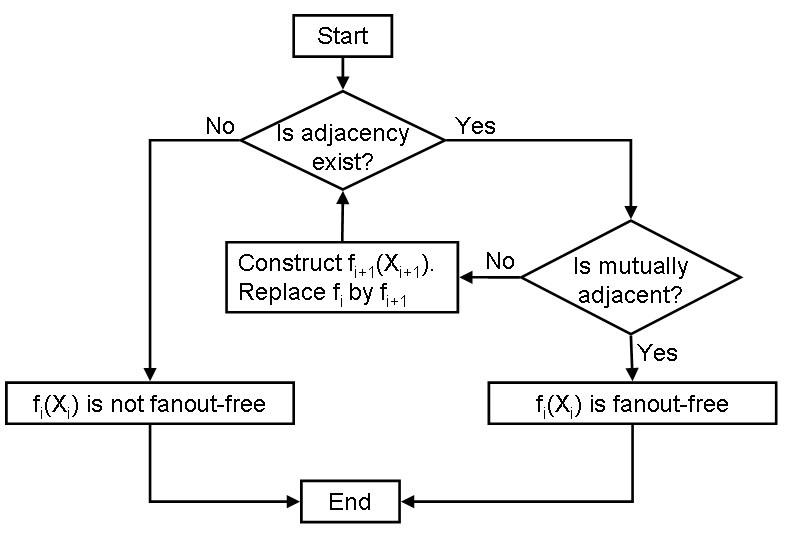
\includegraphics[width=0.55\textwidth,height=\textheight]{./resources/jph.png}
\caption{JPH演算法流程}\label{fig:jph}
}
\end{figure}

\hypertarget{ux65b0ux63d0ux51faux7684ux65b9ux6cd5}{%
\section{新提出的方法}\label{ux65b0ux63d0ux51faux7684ux65b9ux6cd5}}

本篇論文提出的演算法大部分基於JPH演算法。作者推導出了下列disappearance與adjacency之間的等同關係,並根據這個關係,將判斷adjacency的問題化簡為判斷disappearance的問題。

\hypertarget{ux5b9aux7406ux63a8ux5c0e}{%
\subsection{定理推導}\label{ux5b9aux7406ux63a8ux5c0e}}

\begin{lem}[Adjacency implies disappearance]

令$x_i \neq x_j$為$f(X)$之輸入變數。
若$x_i =_a x_j$,
則$x_j$消失於$f(x_i=a)$中,且$x_i$消失於$f(x_j=a)$中。

\end{lem}

上述引理十分直觀,並且可透過反證法證明。它的逆敘述也成立:

\begin{lem}[Disappearance implies adjacency]

令$x_i \neq x_j$為$f(X)$之輸入變數。
若$x_j$消失於$f(x_i=a)$中,且$x_i$消失於$f(x_j=a)$中,
則$x_i =_a x_j$

\end{lem}

上述引理較不直觀,需要透過假設\(f = x_ix_jA + x_iB + x_jC + (x_i+x_j)D + E\)的形式,並利用前提中的「消失」來推導出\(A,B,C,D,E\)中哪些項為\(0\),以此驗證兩個cofactor的確相等。

由上述兩個引理,作者得出adjacency與disappearance等價的結論:

\begin{thm}[Adjacency $\Leftrightarrow$ disappearance]

令$x_i \neq x_j$為$f(X)$之輸入變數。
$x_i =_a x_j$,若且唯若
$x_j$消失於$f(x_i=a)$中,且$x_i$消失於$f(x_j=a)$中。

\end{thm}

\hypertarget{ux6f14ux7b97ux6cd5ux64cdux4f5cux7bc4ux4f8b}{%
\subsection{演算法操作範例}\label{ux6f14ux7b97ux6cd5ux64cdux4f5cux7bc4ux4f8b}}

以下為作者實際示範使用disappearance性質來檢測adjacency關係的例子。令輸入為下列\(f\):

\[f = x_1x_2x_3x_4 + x_1x_2x_3x_5 + x_4x_6 + x_5x_6\]

\begin{enumerate}
\def\labelenumi{\arabic{enumi}.}
\item
  與JPH演算法相同,作者先計算了\(f\)中\(x_1, x_2, \dots, x_6\)的cofactors。

  \[\begin{cases}
  f(x_1 = 0) = x_4x_6+x_5x_6\\
  f(x_2 = 0) = x_4x_6+x_5x_6\\
  f(x_3 = 0) = x_4x_6+x_5x_6\\
  f(x_4 = 0) = x_1x_2x_3x_5+x_5x_6\\
  f(x_5 = 0) = x_1x_2x_3x_4+x_4x_6\\
  f(x_6 = 0) = x_1x_2x_3x_4+x_1x_2x_3x_5
  \end{cases}\]
\item
  接著,作者以列出二維矩陣的方式,來記錄\(x_i\)中是否有出現\(x_j\)。下列矩陣當中,\((i, j)\)項為\(0\)代表\(x_j\)消失於\(f(x_1 = 0)\)的cofactor中;反之則代表有出現。由於cofactor的定義,對角線項全為\(0\)。

  \[\begin{matrix}
  & x_1 & x_2 & x_3 & x_4 & x_5 & x_6\\
  f(x_1 = 0) & \textcolor{gray}{0} & \textcolor{red}{0} & 0 & 1 & 1 & 1\\
  f(x_2 = 0) & \textcolor{red}{0} & \textcolor{gray}{0} & 0 & 1 & 1 & 1\\
  f(x_3 = 0) & 0 & 0 & \textcolor{gray}{0} & 1 & 1 & 1\\
  f(x_4 = 0) & 1 & 1 & 1 & \textcolor{gray}{0} & 1 & 1\\
  f(x_5 = 0) & 1 & 1 & 1 & 1 & \textcolor{gray}{0} & 1\\
  f(x_6 = 0) & 1 & 1 & 1 & 1 & 1 & \textcolor{gray}{0}
  \end{matrix}\]

  若是\((i, j)\)項與\((j, i)\)為\(0\),則由定理可以推出\(x_i =_0 x_j\)。遍歷檢查矩陣中的每一項\footnote{實際上,若\(x_i\)已被劃入某等價類中,則\(f(x_i=a)\)列就不需再檢查一次。},則可以得到所有\(=_1\)的adjacency關係。對\(f(x_i = 1)\)的cofactors重複步驟1與步驟2,則可以得到\(f\)中所有的adjacency
  classes。

  此範例中,變數被分為三個等價類:

  \[\textcolor{red}{\{x_1, x_2, x_3\}} \textcolor{blue}{\{x_4, x_5\}} \{x_6\}\]
\item
  作者按照JPH演算法的函式拆解定理給出新的函式\(g(\phi_1, \phi_2, \phi_3)\)應當滿足的條件:

  \begin{figure}
  \centering
  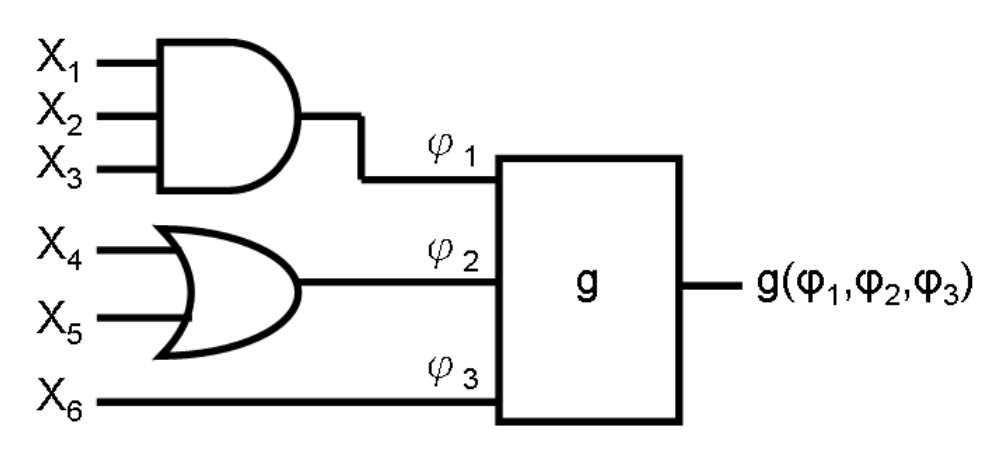
\includegraphics[width=0.55\textwidth,height=\textheight]{./resources/factor.png}
  \caption{\(g\)應滿足的條件}
  \end{figure}

  在JPH中,我們需要建造真值表以尋找符合條件的\(g\),但建造真值表的時間複雜度為\(O(2^N)\),其中\(N\)為變數的數量。這邊作者利用division與absorption
  laws,提出了一個基於替換\(f\)的做法。欲尋找\(g\)的布林表達式,我們只需要在\(f\)中將\(x_i\)替換成它的等價類\(\phi_k\)即可:

  \[\begin{aligned}
  &{} f(x_1, x_2, x_3, x_4, x_5, x_6) = \textcolor{red}{x_1x_2x_3}\textcolor{blue}{x_4}+\textcolor{red}{x_1x_2x_3}\textcolor{blue}{x_5}+\textcolor{blue}{x_4}x_6+\textcolor{blue}{x_5}x_6\\
  & = f(\phi_1, \phi_1, \phi_1, \phi_2, \phi_2, \phi_3) = \textcolor{red}{\phi_1\phi_1\phi_1}\textcolor{blue}{\phi_2}+\textcolor{red}{\phi_1\phi_1\phi_1}\textcolor{blue}{\phi_2}+\textcolor{blue}{\phi_2}\phi_3+\textcolor{blue}{\phi_2}\phi_3\\
  & = g(\phi_1, \phi_2, \phi_3) = \textcolor{red}{\phi_1}\textcolor{blue}{\phi_2} + \textcolor{blue}{\phi_2}\phi_3
  \end{aligned}\]
\end{enumerate}

重複迭代上述三個步驟直到滿足圖~\ref{fig:jph}中的「\(f_i(X_i)\) is
fanout-free」則化簡出的函式為\(f\)的一個fanout-free表示法。若途中遇到無任何adjacency關係的狀況,則\(f\)並不是一個fanout-free的布林函式。

\hypertarget{ux8907ux96dcux5ea6ux5206ux6790}{%
\subsection{複雜度分析}\label{ux8907ux96dcux5ea6ux5206ux6790}}

\begin{itemize}
\item
  JPH演算法:對於每一對變數,等效性檢查的時間複雜度為\(O(2^N)\),其中\(N\)為變數個數。因此,整體時間複雜度為\(O(N^22^N)\)。此為一exponential
  time演算法。
\item
  本文提出算法:建造矩陣過程需要處理\(N\)個cofactors,且每個cofactor中約有\(NK\)個項,故時間複雜度為\(O(N^2K)\)。此為一polynomial
  time演算法。
\end{itemize}

\hypertarget{ux5be6ux9a57ux7d50ux679c}{%
\subsection{實驗結果}\label{ux5be6ux9a57ux7d50ux679c}}

圖~\ref{fig:exp}為文中給出的實驗結果。該表顯示了與JPH演算法相比,本文提出的演算法大幅地減少了執行時間。表中IROF行為另一演算法;雖然執行時間多較本文提出的算法還短,但IROF演算法只能做到判斷\(f\)是否為fanout-free,而不能給出實際的fanout-free表示法,因此本文提出的方法相當具有競爭力。

\begin{figure}
\hypertarget{fig:exp}{%
\centering
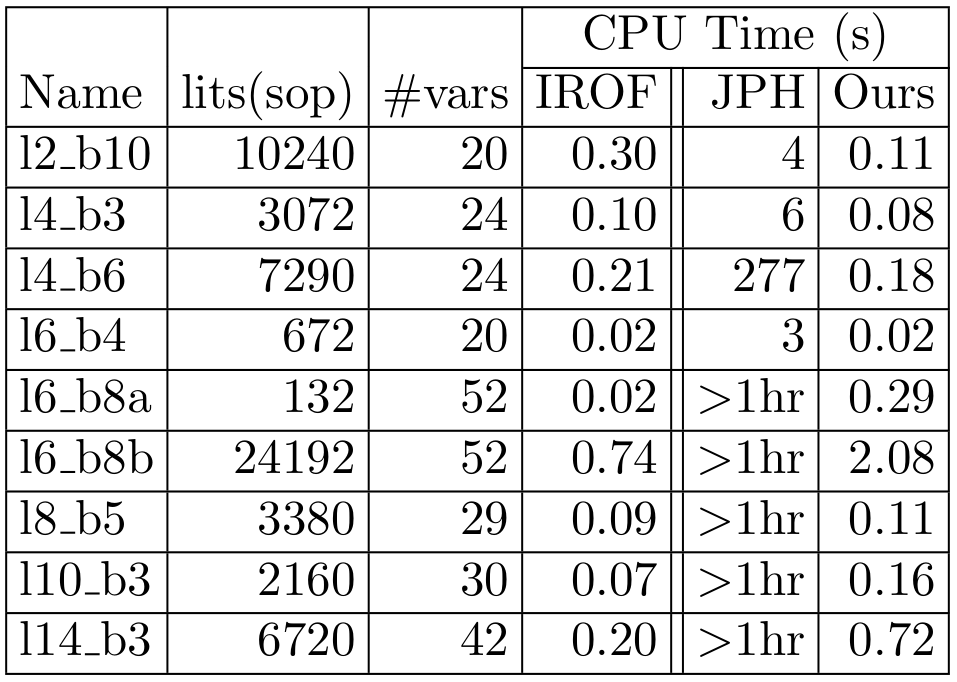
\includegraphics[width=0.55\textwidth,height=\textheight]{./resources/res.png}
\caption{實驗結果}\label{fig:exp}
}
\end{figure}

\hypertarget{ux500bux4ebaux770bux6cd5}{%
\section{個人看法}\label{ux500bux4ebaux770bux6cd5}}

這篇論文提出的方法雖然「簡單」,但背後的洞察(亦即adjacency與disappearance的關係)並不顯然。我十分好奇當時作者如何發現這個潛在的關係。

\hypertarget{refs}{}
\begin{CSLReferences}{0}{0}
\leavevmode\vadjust pre{\hypertarget{ref-4196069}{}}%
\CSLLeftMargin{{[}1{]} }
\CSLRightInline{T.-L. Lee and C.-Y. Wang, {``Recognition of fanout-free
functions,''} in \emph{2007 asia and south pacific design automation
conference}, 2007, pp. 426--431. doi:
\href{https://doi.org/10.1109/ASPDAC.2007.358023}{10.1109/ASPDAC.2007.358023}.}

\leavevmode\vadjust pre{\hypertarget{ref-10.1145ux2f321906.321918}{}}%
\CSLLeftMargin{{[}2{]} }
\CSLRightInline{J. P. Hayes, {``The fanout structure of switching
functions,''} \emph{J. ACM}, vol. 22, no. 4, pp. 551--571, Oct. 1975,
doi:
\href{https://doi.org/10.1145/321906.321918}{10.1145/321906.321918}.}

\end{CSLReferences}

\end{document}
